\section{绘图代码参考}



   注意:在图中的标签一个字母约为 1cm$\times$ 1cm
大小,要注意标签和图形尺寸大小的配合.

如果用在 tex 文件中,直接在工程图片目录下,asy 源文件上加 settings.tex="pdflatex"; \textcolor[rgb]{1.00,0.00,0.00}{文件中的中文用逃逸字符框住\footnote{否则 tex 文件编译报错}},用 
emacs 编译,在 tex 文件中直接加 \verb|\lstinputlisting{源文件名.asy}|,和 \verb$\includegraphics{源文件名}$,即可在修改源代码的同时不改动 TEX 文件。
\clearpage

%%%%%%%%%%%%%%%%%%%%%%%%%%%%%%%%%%%%%%
\subsection{基本命令}

画图时用到的主要有:\textcolor[rgb]{0.00,0.50,0.25}{draw,fill,label,clip,add,shift,rotate }及其扩展命令。
\begin{table}[H]
  \caption{ASY 基本命令}\label{basic_command}
  \begin{tabularx}{14cm}{llp{3cm}}
    \toprule
    % after \\: \hline or \cline{col1-col2} \cline{col3-col4} ...
    功能 & 代码 & 注释 \\
    \midrule
    画笔 & defaultpen(fontsize(100)+linewidth(1pt)+gray(0.5)); & 可自定义 pen 字体大小,线粗大小,绘制颜色 \\
    \rowcolor{lightgray}
    点 & pair x=(1cm,1cm) & 点的坐标 pair(对型) \\
    %线 &  &  \\
    路径 & ((2cm),(1cm))- -((1cm),(1cm)) & - -直线,.. 曲线 \\
     \rowcolor{lightgray}
    绘制 & draw((x,0)--(x,8cm), helpline); & draw(路径,画笔类型) \\
    宏包 & import math & 引入绘制特殊图画的函数包 \\
     \rowcolor{lightgray}
    旋转 & rotate(90,d)*b & 点 b 绕 d 逆时针旋转 90 度得到的点\\
    交点 & extension(a,b,c,d) &  ab 线段与 cd 线段的交点\\
    \rowcolor{lightgray}
    距离 & abs(o - a) &  o 点到 a 点的距离\\
    圆的路径 & circle(o,10cm) &  o 点为圆心,10 cm为半径的圆\\
    \rowcolor{lightgray}
    标签 & label(“字符串”,点,方向) &  字符串如为中文程序前面须加 CJK 的调用命令\\
    \bottomrule
  \end{tabularx}
\end{table}


%%%%%%%%% 画笔设置 %%%%%%%%%%%%%%%%%%%
\subsection{画笔设置}
pen 类型函数:
绘制过程中用的是 currentpen,defaultpen。
过程 defaultpen() 返回当前默认画笔属性。
调用过程 resetdefaultpen() 可重设所有画笔默认属性为初始值。
主要属性包括:字体,线宽,颜色,透明度。
默认颜色名如\ref{colors_name}所示:\\
\begin{description}
  \item[颜色:] 默认的颜色有:\\
\begin{figure}[htbp]
\centering
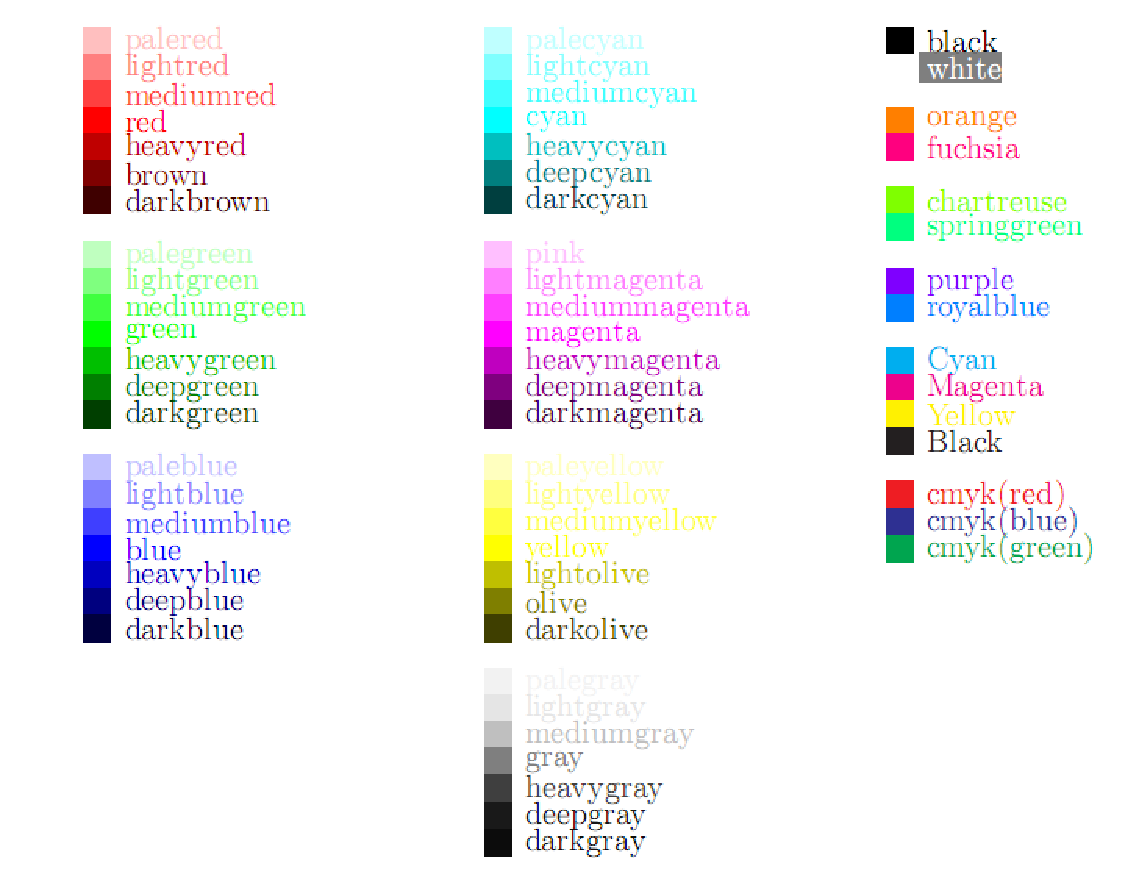
\includegraphics[width=12cm]{colors_name}\\
\caption{asy 各种颜色名称} \label{colors_name}
\end{figure}
  \item[字体:] 默认的字体大小为 12 pt,可以用 defaultpen(pen) 改变。\\
  \fcolorbox{white}{lightgreen}{pen fontsize(real size, real lineskip=1.2*size)}
  \item[线宽:] 默认为 soild 实线类型,0.5dp
  \item[透明度:] opacity 从 0(透明)到 1(不透明)之间先值。
\end{description}
画笔的设置可用如下语句:\\
\fcolorbox{white}{lightgreen}{\parbox{12cm}{
defaultpen(linewidth(0.8)+fontsize(4)+red+opacity(0.5));\\
//设置默认画笔类型\\
pen graypen=linewidth(0.2bp)+gray(0.5);\\
//增加画笔类型
  }}
\clearpage


%%%%%%%%% 点的绘制 %%%%%%%%%%%%%%%%%%%%
\subsection{点的绘制}
%
\subsubsection{空心点,实心点}
dot(参数)表示画实心点;
dot(参数,UnFill)表示画空心点;
参数一般为 pair 二元组的数据类型,表示平面坐标。\\

\lstinputlisting{body/asycode/dots.asy}

\subsubsection{网络格点}
1.自己绘制

\begin{lstlisting}
//`背景网格`
for (int i = 0; i <= 8; ++i) {
  real x = i * cm;
  //`横线`
  draw((0,x)--(8cm,x));
  //`竖线`
  draw((x,0)--(x,8cm));
}
\end{lstlisting}

2.调用 math 模块的 grid 函数\\
\begin{lstlisting}
import math;
add(grid(10,10,gray));
\end{lstlisting}
grid函数使用方法:\\
\begin{lstlisting}
 picture grid(int Nx, int Ny, pen p=currentpen)
\end{lstlisting}


以上为绘制一个 Nx X Ny ,间距为 1 的图形,为 pic 格式。\\
\begin{lstlisting}
add(grid(10,10,gray));
\end{lstlisting}

要使用 grid 函数画的图形,要使用 add(图) 命令,把这个图形加在当前的图上:



\subsubsection{比例分点,中点}
可用这种形式:\textcolor[rgb]{0.00,0.50,0.00}{interp(A,B,t)}
来表示比例分点,其中 t 为比例因子为 real 类型;A,B 为点坐档,pair类型。\\
用 midpoint 函数它们的中点。调用格式是:\textcolor[rgb]{1.00,0.00,0.00}{midpoint(path)},代码如下所示:\\
\begin{lstlisting}
pair X=interp(A,B,t);
pair D=midpoint(A- -B)
\end{lstlisting}


\subsubsection{交点}
调用函数 extension:\\
\begin{lstlisting}
 pair extension(pair P, pair Q, pair p, pair q);
\end{lstlisting}
%
返回线段P\,-\,-\,Q与p\,-\,-\,q延长线的交点,否则,如果两直线平行,返回(infinity,infinity)。

\clearpage

%
%%%%%%%%% 线的绘制 %%%%%%%%%%%%%%%%%%%%
%\subsection{线的绘制}
%
%\subsubsection{实线,虚线}
%代码如下:\\
%
%  \lstinputlisting{body/asycode/lines.asy}
%
%  \begin{description}
%    \item[solid] 可以省略, 表示画实线;
%    \item[dashed ]  画虚线
%    \item[dashdotted] 画点划线
%    \item[dotted ]  画实心点线
%  \end{description}

%\subsubsection{箭头线}
%代码如下:\\
%
%  \lstinputlisting{body/asycode/arrows.asy}
%
%
% \begin{description}
%    \item[Arrow,EndArrow] 效果一样, 都是在路径的末端添加箭头;
%    \item[BeginArrow] 在路径的开头加箭头
%    \item[Arrows] 在路径的头尾都加上箭头
%    \item[MidArrow]  在路径的中间添加箭头
%  \end{description}
%
%\subsubsection{曲线,函数曲线}
%调用 graph 函数,返回类型为 path(guide) 的路径,调用代码格式为:\\
%\begin{center}
%\fcolorbox{white}{lightgreen}{\parbox{12cm}{
%real f(real x)\{return y=x\^{}2;\};\\
%//real x 声明函数自变量 x 是实数型,\\
%//f 前面的 real 声明函数 f 也是一个实数型.\\
%guide graph(real f(real), real a, real b,interpolate join=operator - -);\\
%//描述函数曲线
%  }}
%\end{center}
%
%
%其中:\begin{description}
%        \item[曲线的函数] real f(real x){return y=x}
%        \item[变量范围] a,b
%        \item[画笔线型] 折线:operator - - ;曲线:operator ..
%      \end{description}
%
%  \lstinputlisting{body/asycode/graph_line.asy}\\
%
%\clearpage


%%%%%%%%% 标注 %%%%%%%%%%%%%%%%%%%%
\subsection{标注}
\subsubsection{string 类型}
可包括各种符号,用双引号 " 或单引号 ' 包括起来。空格和换行都会保持不变。
当遇到引号或其他特殊符号时,用\ref{markcode}所示格式进行转义变换。
\begin{table}[htb]
\rowcolors{1}{white}{whiteblue}
\centering
 \caption{ string 类型对应的特殊字符}\label{markcode}
 \begin{tabular}{cc|cc}
  \toprule
    \textbf{换码序列} & \textbf{对应的字符} & \textbf{换码序列} &
    \textbf{对应的字符}\\\midrule
    \verb|\'| & 单引号~\verb|'| & \verb|\"| & 双引号~\verb|"| \\
    \verb|\?| & \verb|?| & \verb|\\| & \verb|\| \\
    \verb|\a| & 报警 & \verb|b| & 退格 \\
    \verb|\f| & 进纸 & \verb|\n| & 换行 \\
    \verb|\r| & 回车 & \verb|\t| & 水平制表符 \\
    \verb|\v| & 竖直制表符 & & \\
    \verb|\0|--\verb|\377| & 八进制编码相应的字符 &
    \verb|\x0|--\verb|\xFF| & 十六进制编码相应的字符 \\
  \bottomrule
 \end{tabular}

\end{table}

\subsubsection{点上的标注}
调用代码如下:

\begin{asycmd}
label(Label,position,align);\\
label("字符串", 点);\\
label("字符串", 点, 方向);\\
Label("字符串",字符旋转方向);\\
label(Label("字符串",字符旋转方向),点,相对点方向);
\end{asycmd}
label 的相对点方向方向有东南西北左中右\textcolor[rgb]{0.00,0.50,0.25}{ LeftSide,RightSide,Center 和 Relative(E或(S,N,W))}\\
Label 的字符旋转方向有东南西北任意角度 \textcolor[rgb]{0.00,0.50,0.25}{Rotate(E或(S,N,W))或 Rotate(x,y)}\\

  \lstinputlisting{body/asycode/label.asy}

\begin{figure}[htbp]
  % Requires \usepackage{graphicx}
  \centering
  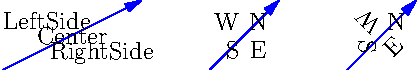
\includegraphics[width=14cm]{body/asycode/label}\\
  \caption{标注方向}\label{label}
\end{figure}


\subsubsection{坐标轴标注}

\begin{lstlisting}
xaxis("$x$",Arrow); //`X 轴下方`
yaxis("$y$",Arrow);//`Y 轴左方` 
\end{lstlisting}



\subsubsection{箭头标注}
\color{red}
\verb|arrow("$t=\frac{1}{3}$",Z,SE);|
\normalcolor

Z 为 pair 类型的点,SE 为相对方向,引号内为标注文字

\subsubsection{中文标注}

在含有中文字符时,前面须加上以下命令:
\begin{lstlisting}
texpreamble("\usepackage{CJK}
 \AtBeginDocument{\begin{CJK*}{GBK}{kai}
   \AtEndDocument{\clearpage\end{CJK*}}");}
\end{lstlisting}

\clearpage


%%%%%%%%% 图形面的绘制 %%%%%%%%%%%%%%%%%%%%
\subsection{面图形的绘制}

\subsubsection{单位圆,单位矩形}
Asymptote 预先定义了很多画基本图形的函数,经常调用的有:\\
\begin{description}
  \item[box] (矩形的左下角, 矩形的右上角);
  \item[ellipse] (椭圆的中心, 水平方向的轴长, 竖直方向的轴长);
  \item[drawline] (直线的第一个点, 直线上的第二个点);
  \item[unitcircle,unitcircle3] 单位圆
  \item[unitsquare,unitsquare3] 单位正方形
  \item[unitsphere] 单位球 - - 3D
  \item[unitbox,unitcube] 正方体 - - 3D
  \item[旋转体函数] 如unitsphere, unitcone, unitcylinder, unitsolidcone,%
  unithemisphere, unitfrustum(real t1, real t2) 等等。
  \item[polygon(n)] 正多边形

\end{description}

  \lstinputlisting{body/asycode/surface.asy}


\begin{figure}[htbp]
  % Requires \usepackage{graphicx}
  \centering
  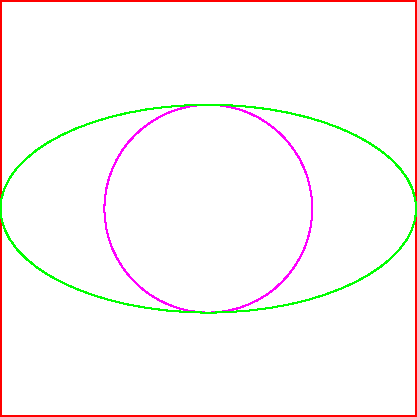
\includegraphics[width=8cm]{body/asycode/surface.pdf}\\
  \caption{对应曲线}\label{surface}
\end{figure}

\subsubsection{封闭曲面}
\clearpage


%%%%%%%%% 图形变换 %%%%%%%%%%%%%%%%%%%%
\subsection{图形变换}
shift,scale,rotate,fill,clip,
\subsubsection{平移,放缩,旋转}
\begin{description}
  \item[平移] shift(x,y)$*$图像
  \item[放缩] xscale(放大倍数)$*$图像: xscale(real x),yscale(real y),scale(real s),scale(real x,real y)
  \item[旋转] rotate(旋转角度, 点坐标),绕点逆时针旋转
  \item[反射] reflect(点a,点b):以 a - - b 为对称轴反射
\end{description}

\subsubsection{填充,裁剪}
\begin{itemize}
  \item add(图像,原点)
  \item add(图像,above=false)
  \item fill(封闭区域,颜色)
  \item filldraw(封闭区域,fillpen=填充颜色,drawpen=路径颜色)
  \item clip(裁剪对象(pic),裁剪路径):裁剪命令处理完后 pic 只剩下裁剪出的部分,可用 add 函数再次加入。
\end{itemize}
\textcolor[rgb]{1.00,0.00,0.50}{picture 类型是一个独立的图,用 draw,filldraw 绘制后不会显示,要显示必须用 add 命令。}


\textcolor[rgb]{0.25,0.50,0.50}{填充阴影}使用 pattern 宏包\\

\begin{minipage}{12cm}
\lstinputlisting{body/asycode/pattern.asy}
\end{minipage}


hatch(NW) 是一种西北走向的阴影斜线的图形; 用\verb$ add("name",hatch(NW))$; 命名为 name。
接下去用 \verb$pattern("name")$ 的方式把它做成一个类似与颜色的画笔。
hatch() 函数还有其他参数, 比如线的粗细, 线的间隔等.



\clearpage


%%%%%%%%% 导入数据 %%%%%%%%%%%%%%%%%%%%
\subsection{导入外部文件}


\subsubsection{导入自定义宏包}
自己做好一些图形后可以将他们保存为模板,方便以后调用,可以将其做成宏包形式,以方便在以后的绘图中导入。

可以将自定义宏包放在和 .asy 代码文件同一文件夹下,或 Asymptote 的安装路径下 \verb$C:\Program Files\Asymptote$

\subsubsection{导入外部数据} 


\subsubsection{导入外部图片} 
